% \chapter{Desenvolvimento/Implementação}\label{cap:development}

% Neste capítulo é descrito o trabalho de implementação, salientando os pontos mais relevantes da mesma, dificuldades  encontradas ou soluções técnicas inovadoras desenvolvidas ou aplicadas.  Em particular, se foi usado código desenvolvido por terceiros (por exemplo, código {\it open-source}), deve ser facilmente distinguível quais as funcionalidades originais do mesmo e o que foi necessário implementar para obter as funcionalidades desejadas.


\chapter{Arquitetura do sistema}\label{cap:development}
Neste capítulo, é abordado em detalhe a arquitetura e a estrutura adotada para a construção dos componentes do sistema. É importante compreender que o sistema foi concebido como um conjunto de módulos, com cada um desempenhando funções específicas, e quando operados em conjunto, esses módulos resultam na realização dos propósitos pensados para o sistema.

O sistema é estruturado fundamentalmente em camadas distintas, o backend, o frontend e o banco de dados.

%TODO Sigla api
O backend funciona como o núcleo do sistema. Sua principal função é a de receber os dados, processá-los conforme as regras estabelecidas nos requisitos e histórias de usuários e, armazená-los de maneira segura no banco de dados. Além das funções de armazenamento e processamento, ao backend também é atribuída a responsabilidade de disponibilizar esses dados por meio de uma interface de programação de aplicações (API), que pode ser acessada utilizando métodos HTTP. Esta API age como um intermediário entre a lógica central do sistema e as interfaces com as quais o usuário final interage, o frontend.

%TODO referencia para princípios de design e data visualization - Talvez referir a outra parte da dissertação que entra em mais detalhes
Por outro lado, o frontend é caracterizado como a interface visual que o usuário final acessa. Serve como meio pelo qual os usuários interagem com o sistema, enviando e recebendo informações. Esta camada é projetada para acessar, recuperar e apresentar os dados processados e armazenados pelo backend de uma maneira intuitiva e amigável, utilizando princípios de design e data visualization.

Como pode ser visto na figura~\ref{fig:systemAchitectureImage}, na planta industrial, onde as máquinas com os sensores se encontram, os sensores enviam os dados para o sistema, que recebe eles por meio do modulo de recebimento de dados e os armazena no banco de dados. O modulo de processamento acessa os dados armazenados para realizar a agregação, e a API gerencia o acesso ao banco de dados, disponibilizando as informações para os usuários no frontend.

\begin{figure}[htbp]
	\centering
	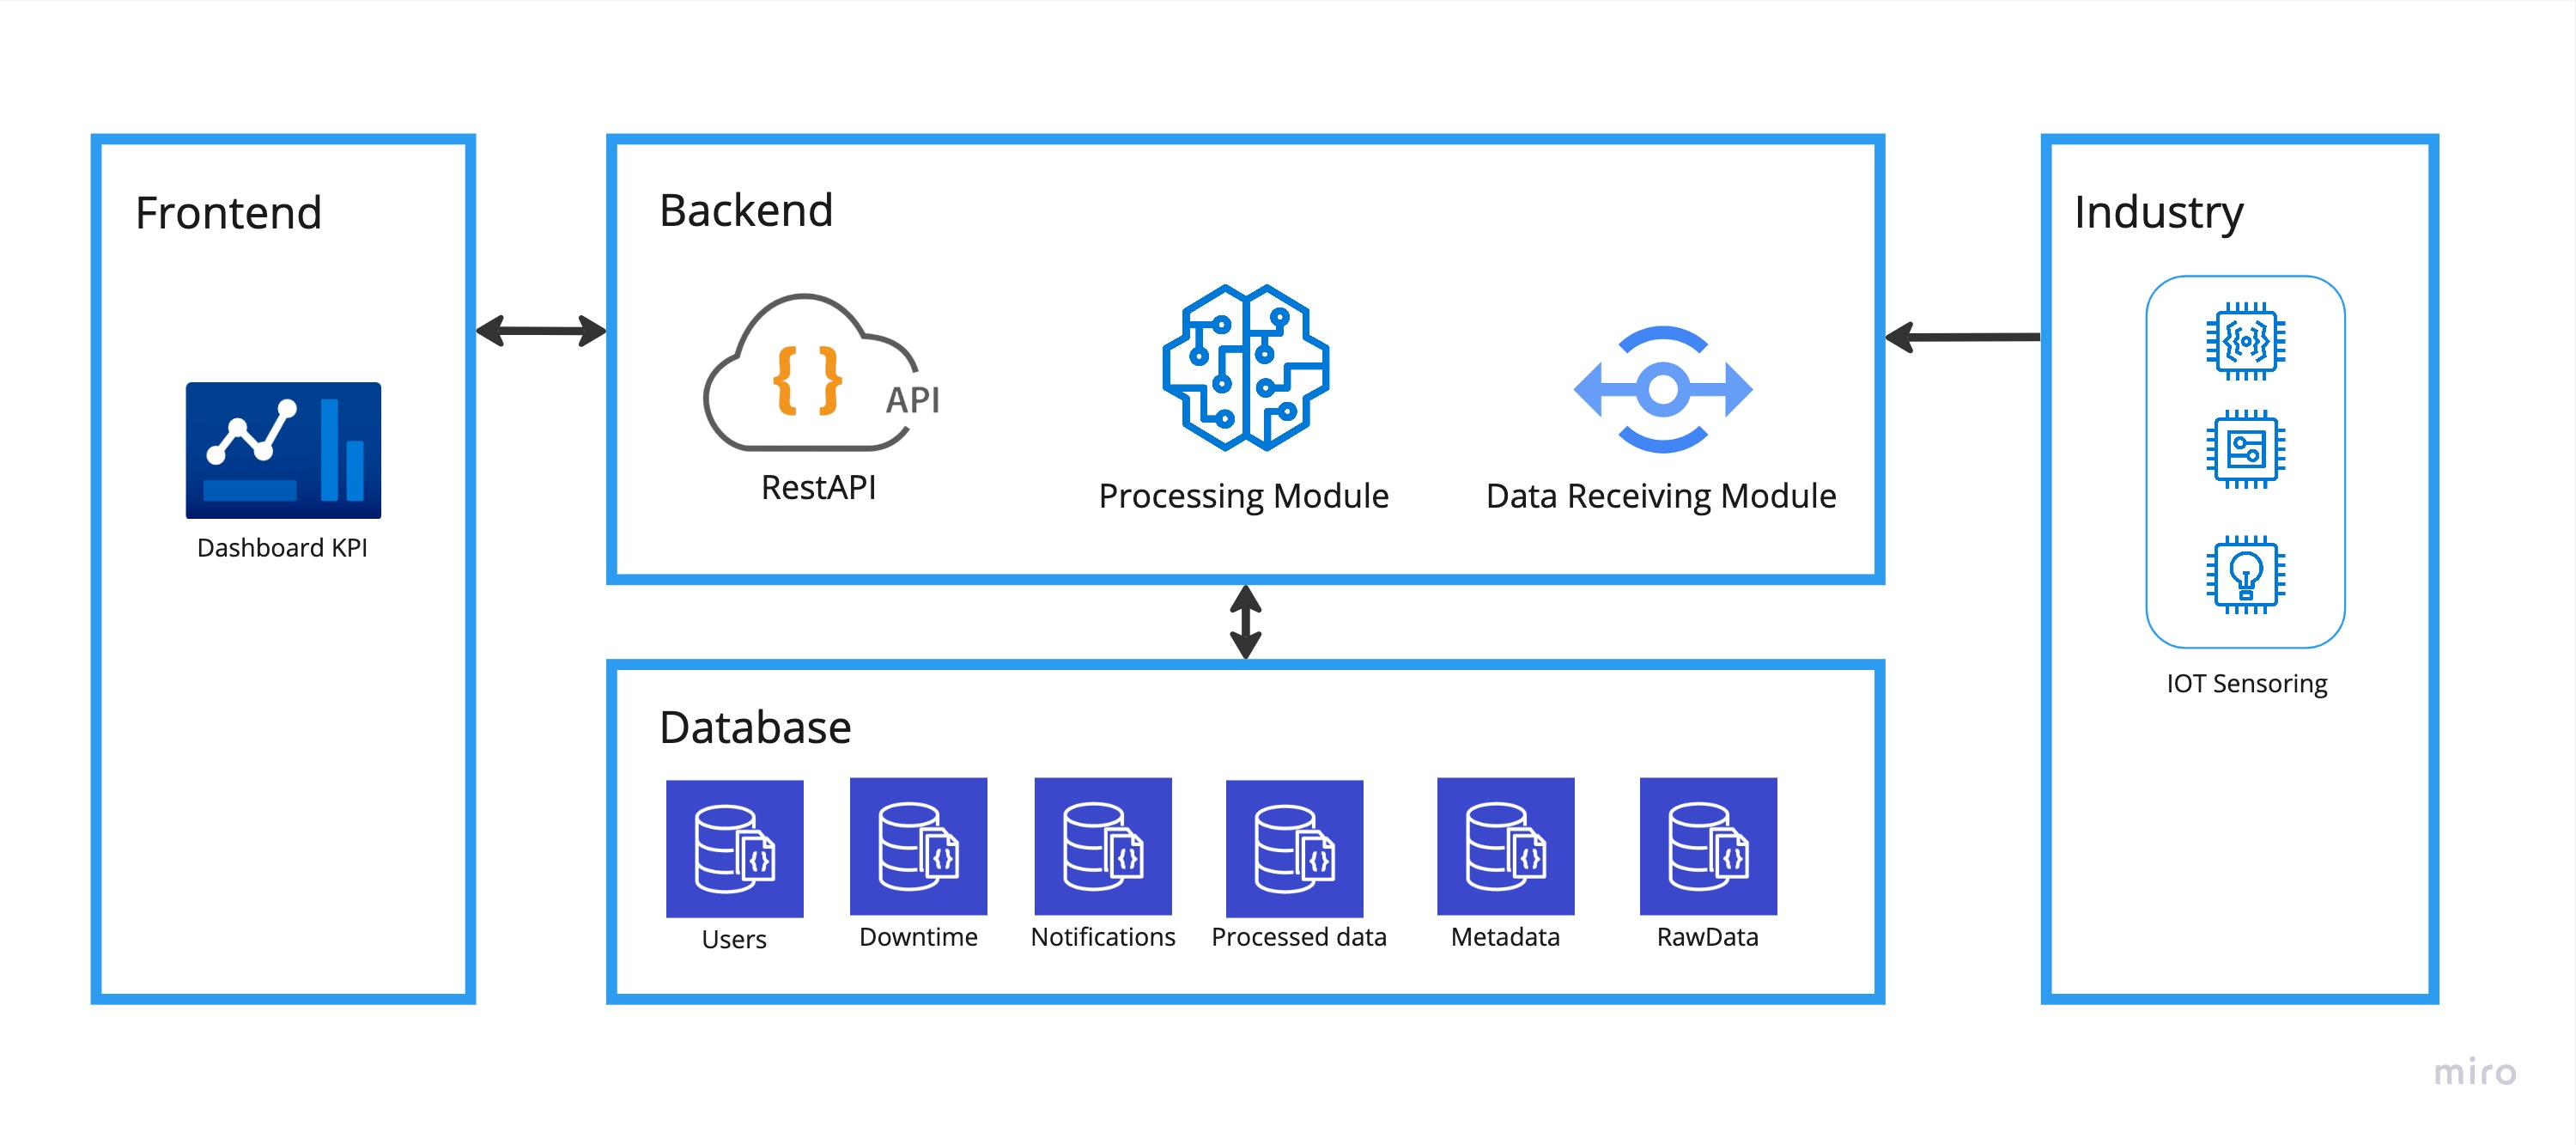
\includegraphics[width=\textwidth]{images/Architecture.jpg}
	\caption{System architecture.}
	\label{fig:systemAchitectureImage}
\end{figure}

Nas seções seguintes, cada um desses componentes será explorado mais profundamente, passando por suas especificidades e interações.


\section[Arquitetura do backend]{Arquitetura backend}

\subsection{Modulo de Recebimento de dados}
Inicialmente, destaca-se a classe \texttt{SensorConnection}, cuja principal função é gerenciar a conexão. Esta classe foi projetada para lidar com tarefas essenciais, como a inicialização e manutenção da conexão. Essa classe faz a transmissão dos dados recebidos à uma função designada \texttt{save\_data\_func},, assegurando que os dados sejam encaminhados para manipulação apropriada.

Na próxima parte da arquitetura, é utilizada a classe \texttt{IotSensorConnection}, que se origina da interface \texttt{IotSensorConnectionInterface}. Esta interface foi criada para garantir a adaptabilidade do sistema, facilitando a integração de diferentes tipos de recebimentos de dados, como por exemplo, uma classe destinada a gerar dados dos sensores em um ambiente de desenvolvimento, onde não há acesso ao sensor real. A classe \texttt{IotSensorConnection}, quando instanciada, é encarregada de estabelecer a conexão, e criar uma nova thread que opera como um ouvinte ativo, monitorando a chegada de novas informações. Ao perceber a recepção de novos dados, a classe direciona estas informações para uma terceira entidade, a qual detém a responsabilidade de aplicar as regras de negócio.

Esta terceira entidade é a classe \texttt{SensorsRepository}, que quando acionada com dados oriundos dos sensores, tem a responsabilidade de avaliar a informação com base nos parâmetros estabelecidos, decidindo se é imperativo acionar um alerta, e tornar os dados do sensor acessíveis via API, garantindo que esses dados estejam disponíveis para serem transmitidos em tempo real, via stream, para todos os usuários conectados. Além do mais, o dado é salvo no banco de dados, especificamente na coleção de dados brutos do data lake, \texttt{Raw Data}. Uma vez salvos no banco de dados, estes dados brutos estão disponíveis para serem processados pelo módulo de agregação.

O diagrama que mostra a organização dessas classes pode ser visto na figura ~\ref{fig:receiveData}. Este design assegura que os dados brutos dos sensores sejam efetivamente recebidos, avaliados e conservados, aprimorando o fluxo de trabalho e maximizando a eficiência operacional.

No capítulo~\ref{cap:implementation}, é aprofundado nos detalhes de implementação desse módulo.


\begin{figure}[htbp]
	\centering
	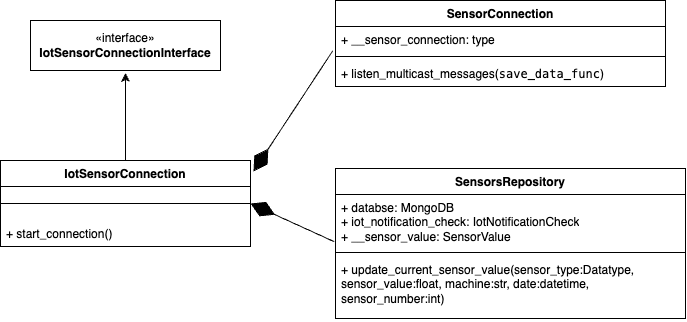
\includegraphics[width=\textwidth]{images/recebimento_dados.png}
	\caption{Module to receive sensor data.}
	\label{fig:receiveData}
\end{figure}

\subsection{API}
- Camada de recebimento das requisições
- Regras de negocio e modelos do sistema
- Camada de infraestrutura


\subsection{Modulo de processamento}


\section[Arquitetura do frontend]{Arquitetura do frontend}
- Next JS e estrutura pre definida de pastas para as paginas do sistema
- Componentes e layouts
- Context API e seu uso
- Acesso a camada externa (API)

\section{Containers}
Explicar sobre os containers

\section{Web Server}
Explicar sobre o NGINX

\section[Princípios do SOLID]{Princípios do SOLID}
Tópicos explicando cada uma das letras do SOLID e relacionando com exemplos concretos do sistema